\chapter{Shaping of Polymers (Verwerken van Kunststoffen)}
Vooraleer we hier echt op ingaan bekijken we eerst wat voor kunststoffen (polymers) er zijn, en wat belangrijke eigenschappen voor het behandelen van deze kunststoffen zijn.
\subsection{Polymers (Kunststoffen)}
Er zijn 3 grote groepen van kunststoffen:
\begin{itemize}
    \item \textbf{Thermoplastics:} Dit zijn (redelijk) lange polymeer ketens, verbonden door secundaire (zwakke) krachten (Van Der Waals), deze krachten zijn makkelijk te verbreken met warmte.
    \item \textbf{Thermosets:} Dit zijn ook lange polymeer ketens, maar deze zijn verbonden door sterke covalente bindingen (cross-links), wat hun eigelijk 3D-moleculen maakt, deze kunnen niet worden verbroken met warmte, als je genoeg opwarmt dan kunnen ze wel chemisch degraderen, verkolen of verbranden ofzo maar ze kunnen niet smelten of zacht worden en kunnen dus niet worden hergebruikt.
    \item \textbf{Elastomers:} Dit zijn eigelijk gewoon 'slechte thermoplastics', ze hebben lange polymeer ketens met een klein aantal van die cross-links, dit maakt hun elastisch, ze kunnnen hierdoor 'unfolden' en terugvouwen, maar ze kunnen ook worden gesmolten en hergebruikt.
\end{itemize}
\begin{figure}[H]
  \centering
  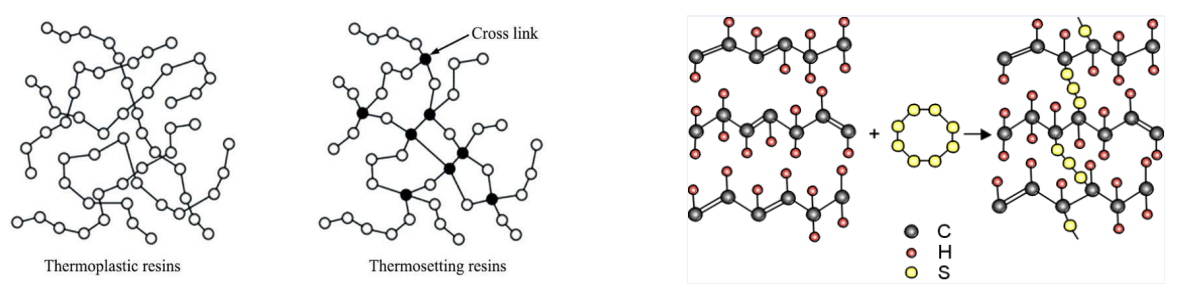
\includegraphics[width=0.8\textwidth]{polymers.png}
  \caption{Polymeerketens}
  \label{fig:polymers.png}
 \end{figure}
 Op de rechtse figuur zie je die gele crosslinks die zorgen voor dat elastisch effect, ze zorgen dat de polymeren niet over elkaar kunnen glijden, gaat terug naar oorspronkelijke vorm (als je toch niet te hard trekt).
 \newpage
 \subsection{Belangrijke eigenschappen voor verwerken van kunststoffen}
 De 2 belangrijkste zijn: heat transfer (warmteoverdracht) en viscosity (viscositeit). We zien deze zometeen, eerst even deze figuur:
\begin{figure}[H]
  \centering
  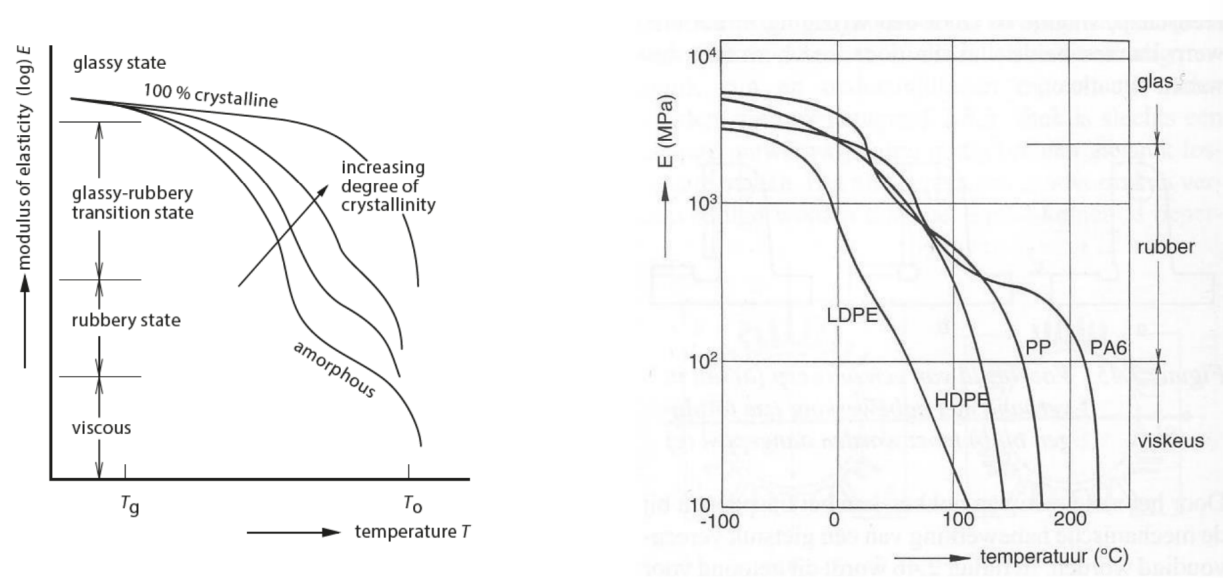
\includegraphics[width=0.8\textwidth]{thermoplasticsgrafieken.png}
  \caption{Grafieken van thermoplastics}
  \label{fig:thermoplasticsgrafieken.png}
 \end{figure}
De \textbf{linkse grafiek} toont de logaritmische elasticiteitsmodulus in functie van de temperatuur, dit laat visueel zien hoe een polymeer bij opwarming transformeert door verschillende materiaaltoestanden: het begint in een harde glastoestand (glassy state), gaat via een overgangsfase (glassy-rubbery transition state) over in een rubberachtige toestand (rubbery state), en smelt uiteindelijk tot een viskeuze, vloeibare toestand (viscous). De pijl toont aan hoe het gedrag veranderd hiervan naarmate de kristalliniteit van het materiaal dus toenoeemt. Belangrijke temperaturen die zijn aangeduid zijn de glastransitietemperatuur (Tg) en de smelttemperatuur (Tm of To).
\newline
De \textbf{rechter grafiek} is een toegepaste versie van de linkergrafiek, de E-modulus is hier uitgezet bij werkelijke temperaturen (van ongeveer -100 °C tot 200 °C), de curves van veel commercieel gebruikte thermoplasten zoals LDPE, HDPE, PP en PA6 worden hier vergeleken met elkaar. De referentiezones 'glas', 'rubber' en 'viskeus' worden hier ook aangegeven zodat je per specifiek materiaal kan aflezen bij welke temperatuur een materiaal zijn stijfheid verliest en vloeibaar wordt.
\newpage
\subsubsection{Heat Transfer (Warmteoverdracht)}
Dan nu warmteoverdracht, dit is natuurlijk een belangrijk concept want om kunststoffen te kunnen verwerken moeten we ze opwarmen, en om ze te kunnen afkoelen moeten we warmte kunnen afvoeren
 , er zijn 3 verschillende mechanismen van warmteoverdracht: Conductie, Convectie en Straling. (gezien bij Thermal Technologies)
\subsubsection{Warmtegeleiding (Thermal Conduction) \textbf{en} het Fourier-getal}
Polymeren hebben typisch een trage warmtegeleiding (warmte geleidingscoëfficiënt $k \approx 0.2 W/mK$ en thermische diffusiviteit $\alpha \approx 0.1 mm^2/s$), oftewel meer zichtbaar met de volgende formules:
\begin{align*}
  Q &= -kA \frac{\partial T}{\partial x} \\
\end{align*}
De formule hierboven is \textbf{stationair}, dit betekent dat de temperatuurverdeling in het materiaal niet verandert in de tijd, er is dus een constante warmteflux $Q$ door het materiaal. De formule geeft aan dat de warmteflux $Q$ evenredig is met de oppervlakte $A$ en de temperatuurgradiënt $\frac{\partial T}{\partial x}$, en omgekeerd evenredig is met de warmtegeleidingscoëfficiënt $k$. Een hogere waarde van $k$ betekent dat het materiaal beter warmte geleidt, terwijl een lagere waarde betekent dat het materiaal een betere isolator is.
\newline
\begin{align*}
    \frac{\partial^2 T}{\partial x^2} &= \alpha \frac{\partial T}{\partial t}
\end{align*}
De formule hierboven is \textbf{transient}, dit betekent dat de temperatuurverdeling in het materiaal verandert in de tijd, $\alpha$ is hier de thermische diffusiviteit, die aangeeft hoe snel warmte zich door het materiaal verspreidt. Een hogere waarde van $\alpha$ betekent dat het materiaal sneller opwarmt of afkoelt, terwijl een lagere waarde betekent dat het materiaal langzamer reageert op temperatuurveranderingen.
\newline
De thermische diffusiviteit $\alpha$ kan worden berekend met de volgende formule:
\begin{align*}
    \alpha = \frac{k}{\rho c_p}
\end{align*}
Hierbij is $\rho$ de dichtheid van het materiaal en $c_p$ de specifieke warmtecapaciteit. Deze formule geeft aan dat de thermische diffusiviteit afhankelijk is van zowel de warmtegeleidingscoëfficiënt als de thermische massa van het materiaal (product van dichtheid en specifieke warmtecapaciteit). Rho en $c_p$ samen zijn iets volumetrischs, ze geven aan hoeveel warmte er nodig is om een bepaald volume van het materiaal op te warmen.
\newline
Het Fourier-getal ($Fo$) is een dimensionloos getal dat de verhouding aangeeft tussen de tijd die nodig is voor warmte om zich door een materiaal te verspreiden en de tijd die nodig is voor het materiaal om op te warmen of af te koelen. Het wordt gedefinieerd als:
\begin{align*}
    Fo = \frac{\alpha t}{L^2}
\end{align*}
Hierbij is $t$ de tijd, $L$ een karakteristieke lengte (zoals de dikte van het materiaal, meestal nemen we de smalste dikte), dit is een dimensieloos getal en $\alpha$ de thermische diffusiviteit. Een hoger Fourier-getal betekent dat warmte sneller door het materiaal verspreidt in vergelijking met de tijd die nodig is om op te warmen of af te koelen, terwijl een lager Fourier-getal betekent dat warmte langzamer verspreidt. Dit is zeer belangrijk in een gesloten mal proces (injection molding).
\newline
Tijd voor complete solidificatie (afkoeling) kan worden geschat met de volgende formule:
\begin{align*}
    t_s \approxeq {3L^2}
\end{align*}
Dus een dubbele dikte resulteert in een 4 keer langere solidificatie tijd, daarom hebben we niet graag te dikke wanden in injection moulding, we willen de dikte beperken.
\subsubsection{Convectie en Straling (Convective and Radiative Heat Transfer)}
In de vloeistof toestand van het polymeer kan warmte worden overgedragen worden door convectie, dit is echter beperkt (bij thermoharders) of zelfs volledig afwezig (bij thermoplasten). Maar als de vloeistof mechanisch gedwongen wordt om te bewegen zoals tijdens het injecteren bij een matrijs of bij extrusie, heeft dit wel een grotere rol.
\newline
Deze warmteoverdracht wordt beschreven door de volgende formule:
\begin{align*}
    Q = \rho C_p u A
\end{align*}
Dit wordt ook de 'Flow heat transfer' genoemd, hier is $u$ de stroomsnelheid van de vloeistof, $A$ het doorsnedeoppervlak van de vloeistof, $\rho$ de dichtheid en $C_p$ de specifieke warmtecapaciteit. 
\newline
Bij het oppervlak zelf is er ook nog warmteoverdracht door convectie (dit is de warmteoverdracht tussen het oppervlak van het materiaal en de omringende lucht of een koelmiddel), dit wordt beschreven door de volgende formule:
\begin{align*}
    Q = h A (T_s - T_0)
\end{align*}
Dit is vooral door de vacuumvorming, deze trekt de opgewarmde lucht weg van het oppervlak, zie volgende foto waar dit duidelijker is:
\begin{figure}[H]
  \centering
  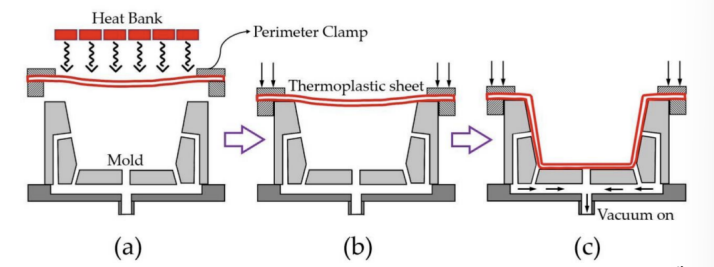
\includegraphics[width=0.6\textwidth]{vacuumheattransfer.png}
  \caption{Vacuumvorming en warmteoverdracht}
  \label{fig:vacuumheattransfer.png}
 \end{figure}
Er is ook nog sprake van warmteoverdracht door straling, beschreven door:
\begin{align*}
    Q = A \sigma T^4
\end{align*}
\subsubsection{Biot modulus}
De biot-modulus bepaalt hoe de temperatuurgradiënt in het materiaal zich ontwikkelt, het is de verhouding tussen hoe snel de warmte aan het oppervlak wordt afgevoerd, gedeeld door de warmtetransport binnen in het materiaal, beschreven door de volgende formule:
\begin{align*}
    Bi = \frac{hL}{k}
\end{align*}
De volgende figuur toont het verschil tussen een kleine en grote biot-modulus, bij een kleine heb je dus een kleine temperatuurgradiënt, dus een soort van evenwicht tussen opwarmen en afkoelen eigelijk, dit is \textit{'dimensionaal stabiel'} (dit betekent dat het materiaal overal ongeveer dezelfde temperatuur heeft tijdens het proces), dit zorgt dus voor \textit{'limited warping'} (zien we later), bij een grote biot-modulus heb je grote temperatuurverschillen \textit{in de directie van de dikte}, een grote temperatuurgradiënt dus, wat voor \textit{'residual thermal stresses'} (dit zijn spanningen die ontstaan door temperatuurverschillen in het materiaal) zorgt, hier is ook een grote kans op 'warping'.
\begin{figure}[H]
  \centering
  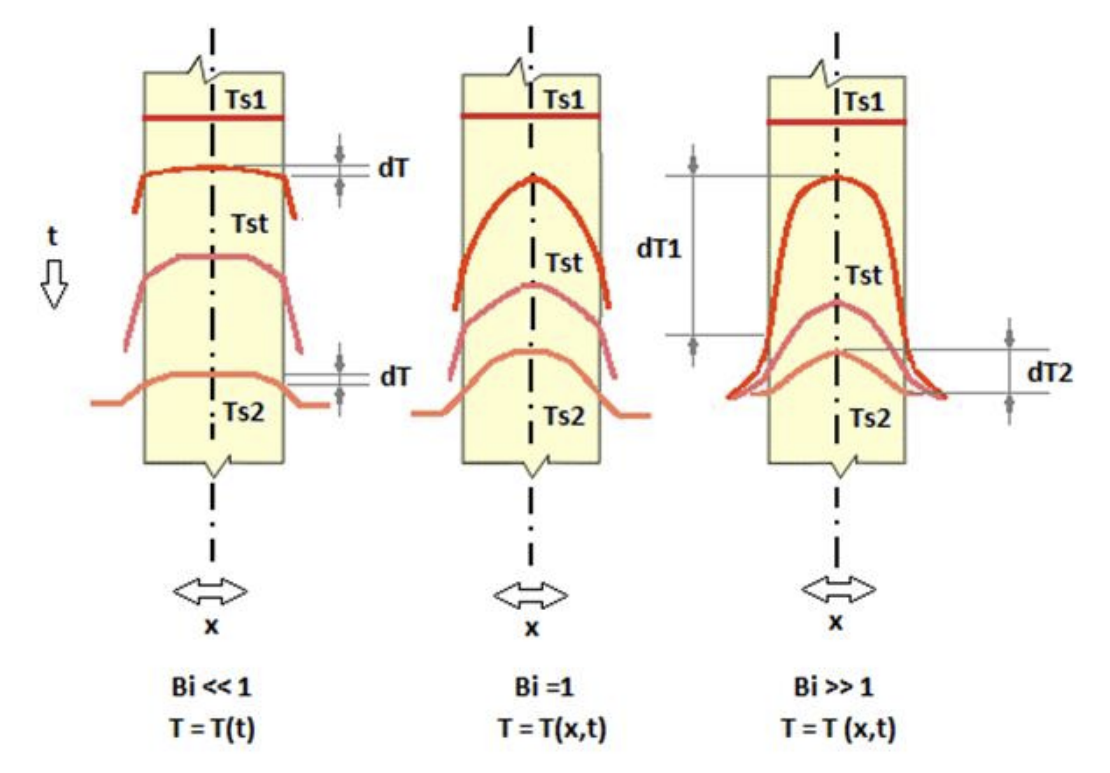
\includegraphics[width=0.6\textwidth]{biot.png}
  \caption{Kleine en grote biot modulus}
  \label{fig:biot.png}
 \end{figure}
\subsubsection{Viscositeit: temperatuur afhankelijkheid}
In gesmolten toestand hebben polymeren een hoge viscositeit, tot wel 1000 Pa.s, bij water of gesmolten metalen is dit juist heeel laag. Er is een relatie tussen temperatuur en viscositeit die wordt beschreven met een exponentiële formule:
\begin{align*}
    \eta(T) = \eta_0 e^{\frac{E_a}{RT}}
\end{align*} 
Hierbij is $\eta(T)$ de viscositeit bij temperatuur $T$, $\eta_0$ een referentie viscositeit, $E_a$ de activeringsenergie voor stroming, $R$ de universele gasconstante en $T$ de absolute temperatuur. Deze formule geeft aan dat de viscositeit van een polymeer exponentieel afneemt met toenemende temperatuur, wat betekent dat het materiaal gemakkelijker stroomt bij hogere temperaturen. Dit is cruciaal voor processen zoals extrusie en spuitgieten, waar het materiaal in gesmolten toestand moet worden verwerkt.
\subsubsection{Viscositeit: afschuifafhankelijkheid (Shear rate dependence)}
Wat we ook kunnen doen is de afschuifsnelheid varieren, want met het model van Carreau-Yasuda werd aangetoond dat de viscositeit ook afhankelijk is van de afschuifsnelheid, beschreven door de volgende formule:
\begin{figure}[H]
  \centering
  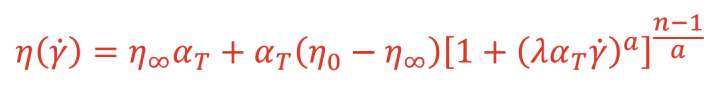
\includegraphics[width=0.8\textwidth]{carreayasuda.png}
  \caption{}
  \label{fig:carreayasuda.png}
 \end{figure}
Met:
\begin{figure}[H]
  \centering
  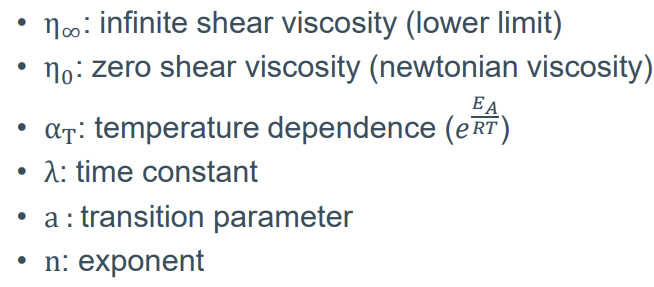
\includegraphics[width=0.5\textwidth]{yassuda.png}
  \caption{}
  \label{fig:yassuda.png}
 \end{figure}
Dit model is makkelijker in te zien en te beschrijven met de volgende grafiek:
\begin{figure}[H]
  \centering
  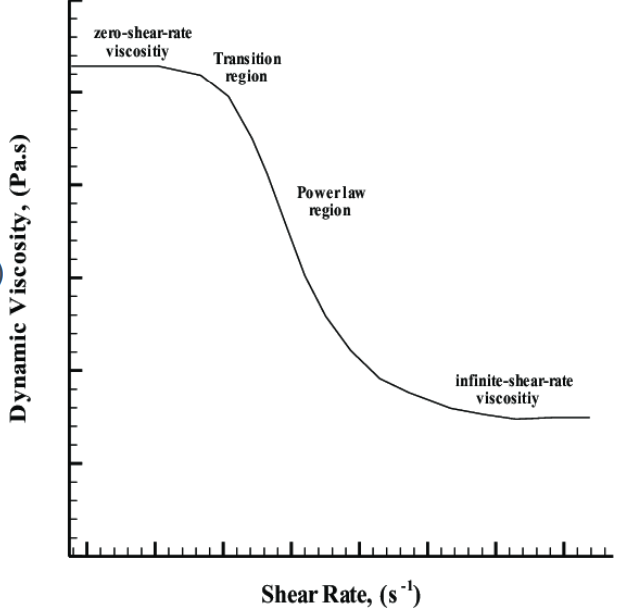
\includegraphics[width=0.6\textwidth]{viscositeitgrafiek.png}
  \caption{Plot van de viscositeit in functie van de afschuifsnelheid}
  \label{fig:viscositeitgrafiek.png}
 \end{figure}
De grafiek toont dat wanneer de afschuifsnelheid toeneemt, de dynamische viscositeit daalt, in de praktijk is dit nuttig want een lagere viscositeit maakt het makkelijker om eem matrijs te vullen. Er is wel een limiet op de grafiek die we kunnen zien, naarmate we de afschuifsnelheid doen toenemen is er uiteindelijk niet meer een significante afname in viscositeit, dit is de zogenaamde 'infinite shear viscosity' ($\eta_\infty$), dit is de minimale viscositeit die het materiaal kan bereiken bij zeer hoge afschuifsnelheden. Deze limiet proberen we te ontwijken want het zorgt voor schade aan het materiaal.
\subsubsection{Andere beïnvloedende factoren (Factors influencing rheology)}
'Rheology' is een algemene term die verwijst naar de studie van de mechanica van vaste stoffen en vloeistoffen.(vooral vloeistoffen)
\newline
Bij het ontwerpen is er altijd een trade-off tussen verwerkbaarheid en prestaties. De viscositeit wordt verder nog beïnvloed door:
\begin{itemize}
  \item \textbf{Molecuulgewicht en de verdeling daarvan:} Een hoger molecuulgewicht leidt tot een hogere viscositeit, omdat langere polymeerketens meer onderlinge interacties hebben, wat de stroomweerstand verhoogt. De verdeling van molecuulgewichten (hoe breed of smal deze is) kan ook invloed hebben op de viscositeit, een bredere verdeling kan leiden tot een complexere stroming.
  \item \textbf{Vertakking in de polymeerketens (Branching):} Meer vertakkingen in de polymeerketens kunnen de viscositeit verhogen, omdat ze de mobiliteit van de ketens verminderen en meer onderlinge interacties veroorzaken.
  \item \textbf{Additieven:} Additieven zoals vulstoffen, weekmakers en stabilisatoren kunnen de viscositeit van een polymeer beïnvloeden. Vulstoffen kunnen bijvoorbeeld de viscositeit verhogen door de interacties tussen de polymeerketens te versterken, terwijl weekmakers de viscositeit kunnen verlagen door de ketens flexibeler te maken.
\end{itemize}
\begin{figure}[H]
  \centering
  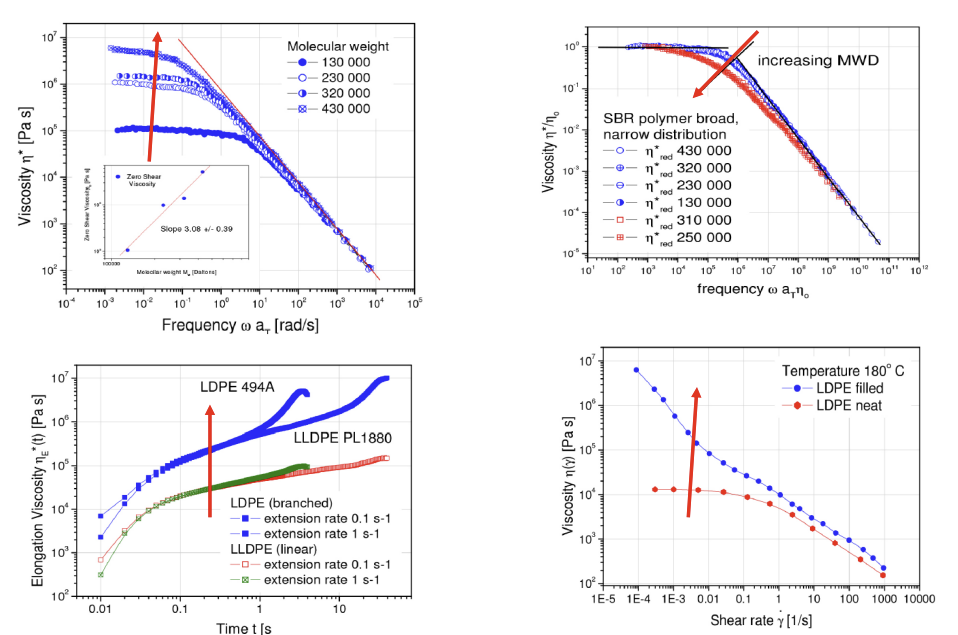
\includegraphics[width=0.8\textwidth]{anderefactoren.png}
  \caption{Andere invloedende factoren op de viscositeit}
  \label{fig:anderefactoren.png}
 \end{figure}
\subsection{Verwerken van thermoplasten (Injection Moulding)}
Injection moulding is één van de meest gebruikte methoden voor het verwerken van thermoplasten, het bestaat uit de volgende stappen:
\begin{itemize}
	\item \textbf{1. Toevoer:} Plastic korrels (pellets) worden vanuit een trechter in de cilinder van een verwarmde extruder gevoerd.
	\item \textbf{2. Transport en smelten:} Een roterende schroef beweegt het materiaal naar voren in de verwarmde cilinder, hierdoor verwarmt het materiaal ook extra (intern) door de schuifkrachten van de roterende schroef.
	\item \textbf{3. Verzamelen:} Het materiaal hoopt zich op voor de schroef (terwijl dat de schroef roteert, beweegt deze daardoor langzaam naar achteren)
\end{itemize}
\begin{figure}[htbp]
  \centering
  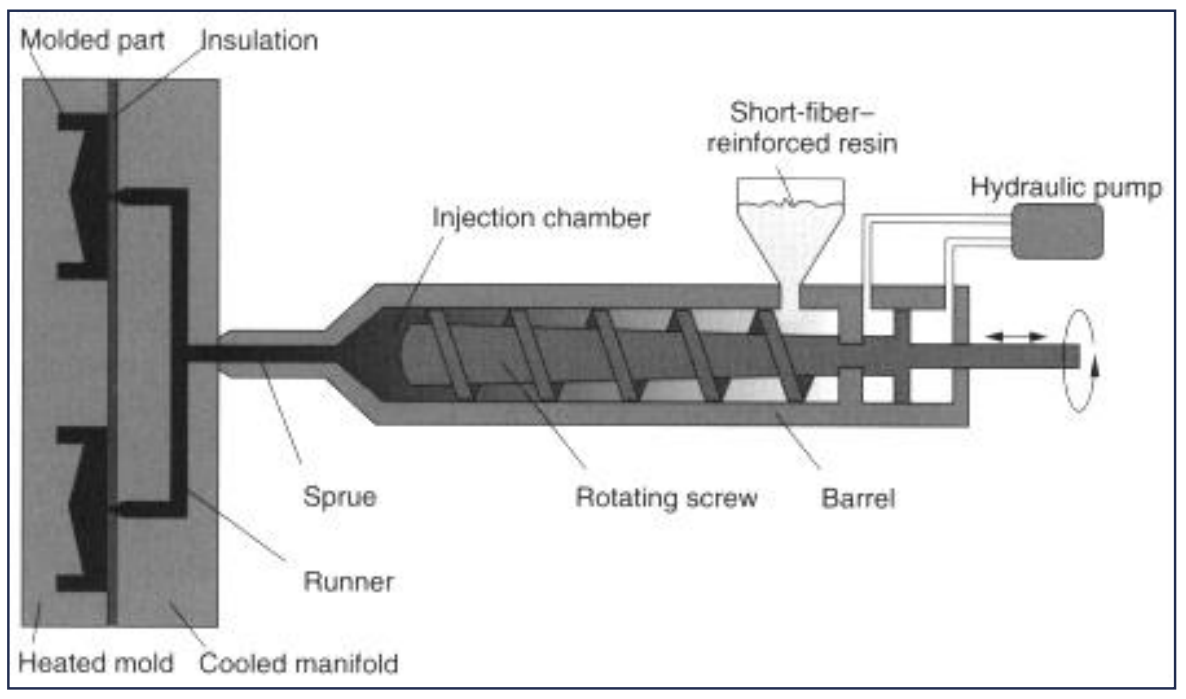
\includegraphics[width=0.5\textwidth]{IM1.png}
  \caption{Moulding proces}
  \label{fig:IM1.png}
\end{figure}
\begin{itemize}
    \item \textbf{4. Injectie:} Wanneer de juiste hoeveelheid materiaal vooraan is verzameld, wordt de plunjer (ram) naar voren geduwd om het materiaal in de mould (matrijs) te spuiten. Omdat dit materiaal zo heet is en de matrijs koud is om snel af te koelen, worden er heel hoge drukken van 200 tot 400MPa gebruikt om het materiaal snel en volledig in de matrijs te krijgen voordat het stolt.
	\item \textbf{5. Stollen:} De matrijs wordt op een lage temperatuur gehouden voor de solidificatie (stollen) van het materiaal.
	\item \textbf{6. Druk behouden:} Eerder gezegd maar, tijdens het koelen wordt de druk op de matrijs behouden.
	\item \textbf{7. Terugtrekken plunjer:} Na volledige stolling beweegt de plunjer terug naar achteren.
	\item \textbf{8. Uitwerpen:} Wanneer het onderdeel voldoende is afgekoeld, opent de matrijs en wordt het onderdeel uitgeworpen.
	\item \textbf{9. Volgende cyclus voorbereiden:} Ondertussen verzamelt zich alweer nieuw materiaal in de injectiekamer voor de volgende productiecyclus.
\end{itemize}
\begin{figure}[htbp]
  \centering
  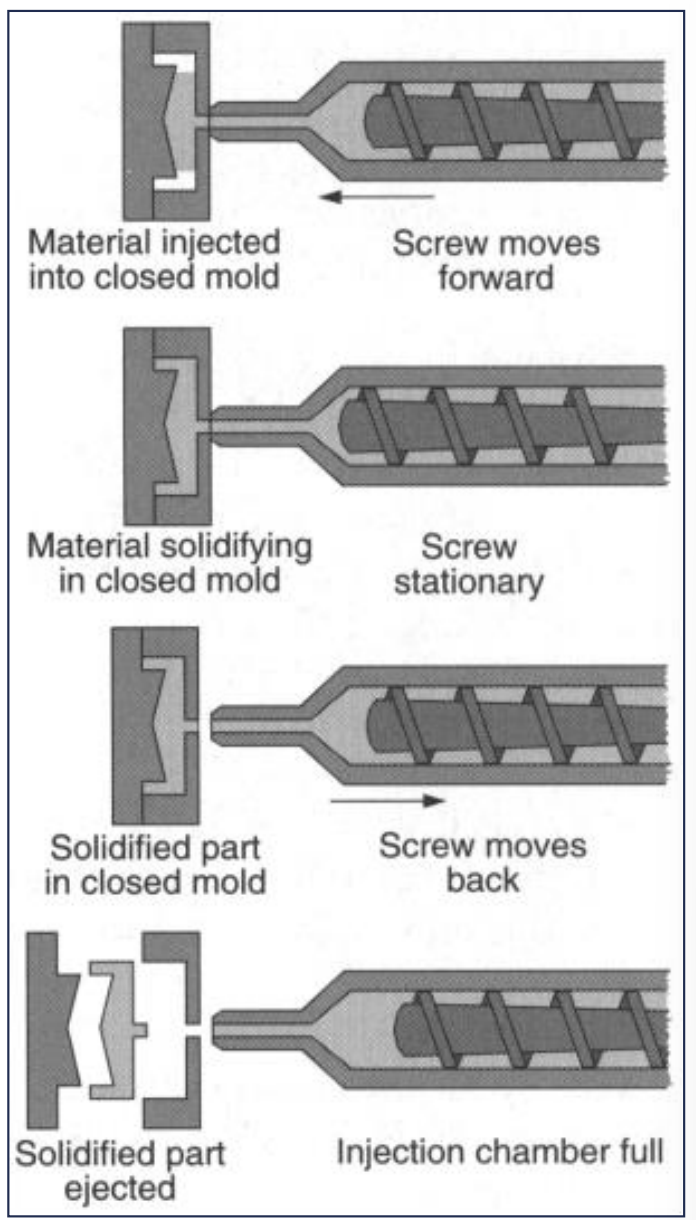
\includegraphics[width=0.3\textwidth]{IM2.png}
  \caption{Injectie proces}
  \label{fig:IM2.png}
 \end{figure}
\newpage
\subsubsection{Cyclus tijd en injectie onderdeel}
De cyclustijd wordt onderverdeeld in een aantal dingen zoals we op de volgende figuur zien:
\begin{figure}[H]
  \centering
  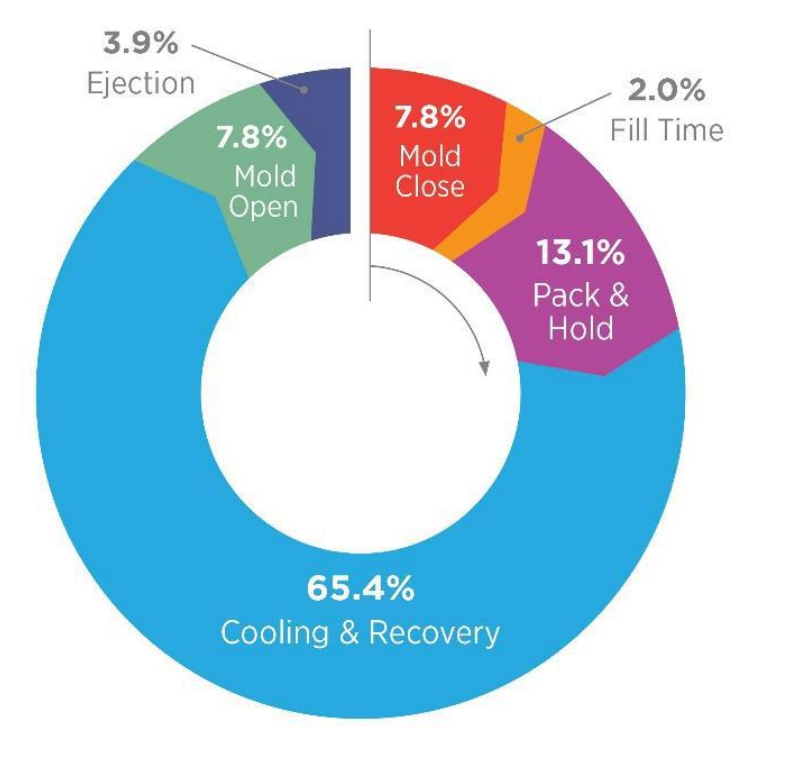
\includegraphics[width=0.35\textwidth]{cyclustijd.png}
  \caption{Cyclustijd}
  \label{fig:cyclustijd.png}
 \end{figure}
 We zien hier dat het afkoelen en tegelijk het verzamelen van nieuw materiaal het langste duurt 65,4\%.
Het injecteren zelf van het materiaal is de kortste stap, overige tijd wordt gespendeerd aan de nadruk, het sluiten en openen van de matrijs en het uitwerpen van het product. Een cyclus zelf kan erg snel zijn, vaak in de grootteorde van enkele seconden. Voor productie is het interessant om ook zo veel mogelijk producten te produceren in een cyclus, daarom wordt een matrijs met meerdere 'cavities' (holtes) gebruikt, verbonden door 'runners' en 'gates', de 'sprue' is de centrale opening waar het gesmolten materiaal binnenkomt, van daaruit stroomt het door de 'runners' naar de 'gates', die het materiaal in de verschillende 'cavities' injecteren waar de onderdelen worden gevormd.
\begin{figure}[H]
  \centering
  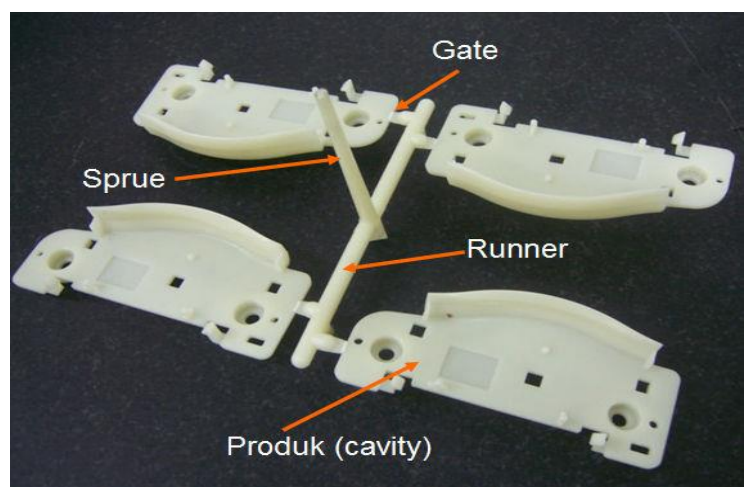
\includegraphics[width=0.5\textwidth]{cavities.png}
  \caption{Cavities}
  \label{fig:cavities.png}
 \end{figure}
 Er is echter een hoge druk nodig om het materiaal effectief tot in elk hoekje van de caviteit te persen, ook moet alle aanwezige lucht naar buiten kunnen ontsnappen, hiervoor worden smalle spleetjes in de matrijs ontworpen (smal zodat als materiaal erdoor gaat, het instant stolt), dit vereist hoge toleranties wat de reden is waarom spuitgietmatrijzen zo duur zijn.
 \subsection{Proces cyclus}
 We zagen eerder de proces stappen van injection moulding, nu gaan we het spuitgietproces zelf in detail is bekijken aan de hand van een grafiek die de positie van de plunjer (ram) en de druk in de matrijs uitzet tegen de tijd:
 \begin{figure}[H]
   \centering
   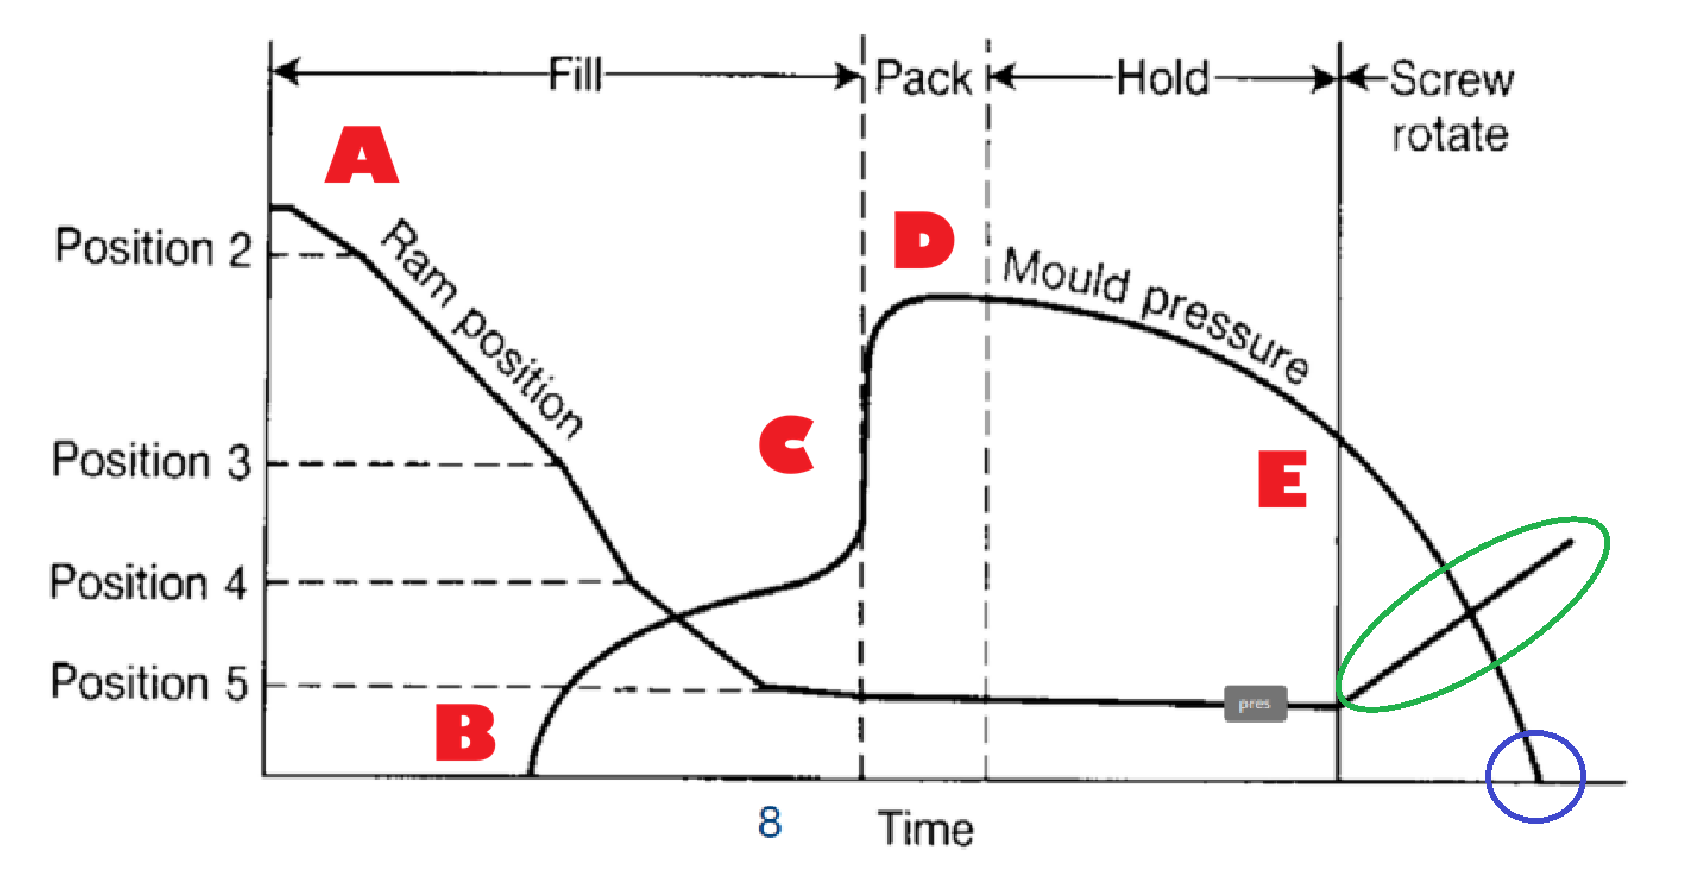
\includegraphics[width=0.6\textwidth]{procescyclus.png}
   \caption{Proces cyclus van injection moulding}
   \label{fig:procescyclus.png}
  \end{figure}
In fase A gaat dus de plunjer naar voor om het hete materiaal in te spuiten, in fase B begint het materiaal de caviteit van de matrijs te vullen, in fase C is de caviteit vol, hierdoor ontstaat een plotselinge zeer snelle druk stijging in de matrijs, dit is het moment waarop eigelijk de injectiedruk van de machine direct wordt overgedragen op de matrijs, in fase D stopt de injectie maar houdt de machine de druk op de matrijs nog steeds hoog zodat er nog een beetje extra materiaal in de matrijs geperst wordt om zo de eerste krimp tijdens het stollen op te vangen, in fase E is de uiterste smalle ingang van de matrijs volledig gestolt, hierdoor wordt het product in de matrijs volledig afgesloten van de druk van de machine, vanaf dit moment gebeuren 2 dingen tegelijk, namelijk dat de plunjer zich terugtrekt (in het groen omcirkelt) en de schroef terug begint te roteren om nieuw materiaal voor de volgende cyclus op te bouwen en dat het materiaal in de matrijs verder afkoelt en begint te krimpen waardoor de druk in de matrijs daalt tot die nul is, dit is het moment dat het product fysiek loskomt van de wand (dit is in het blauw omcirkelt).
\newline
Hier is een versimpelde versie van de bovenstaande figuur, opgesplits in 2 aparte grafieken: 
\begin{figure}[H]
  \centering
  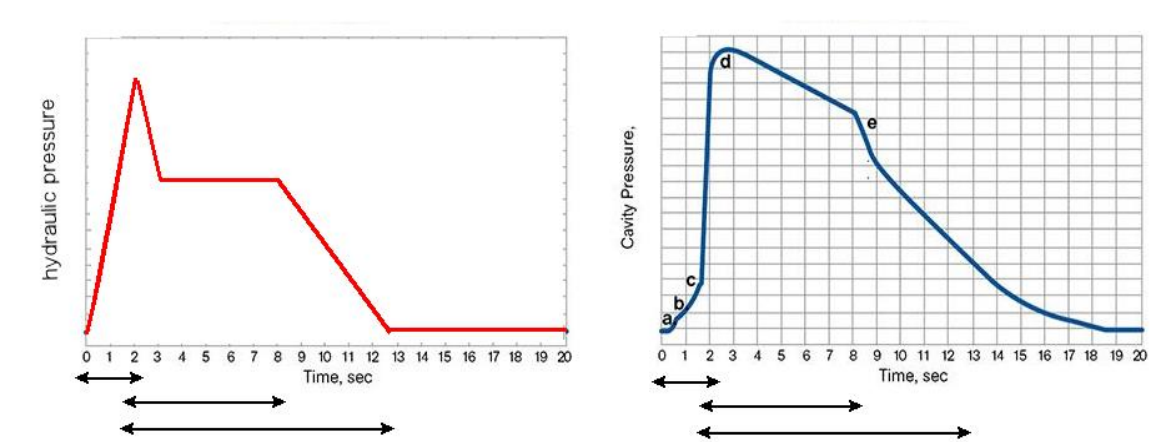
\includegraphics[width=0.8\textwidth]{versimpelde.png}
  \caption{Versimpelde proces cyclus}
  \label{fig:versimpelde.png}
 \end{figure}
\subsubsection{Pressure-Volume-Temperature Cyclus}
We gaan nu is kijken naar het thermodynamische gedrag van een polymeer (in de volgende grafiek gaat dit om polystyreen) tijdens de volledige spuitgietcyclus, hier wordt het specifieke volume ($cm^3/g$) uitgezet tegen de temperatuur.
\begin{figure}[H]
  \centering
  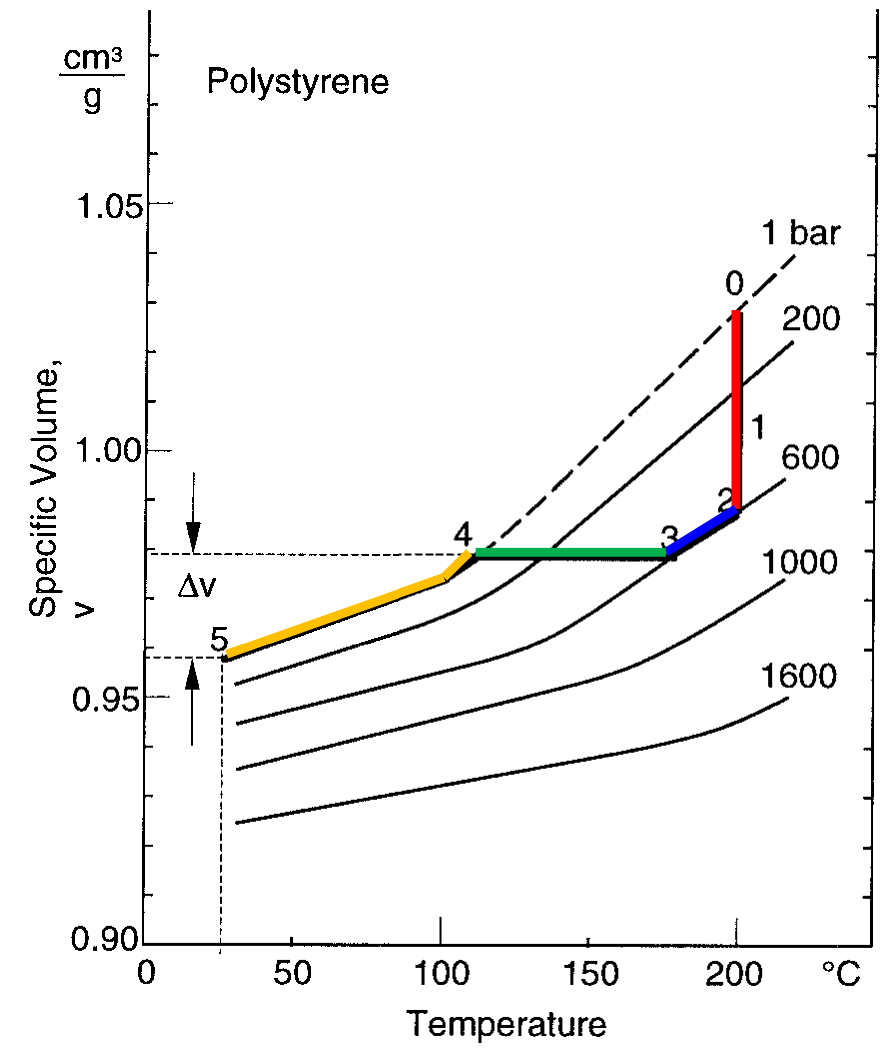
\includegraphics[width=0.4\textwidth]{PVT.png}
  \caption{Pressure-Volume-Temperature Cyclus van polystyreen}
  \label{fig:PVT.png}
 \end{figure}
Het proces is opgedeelt in 4 stappen:
\begin{itemize}
    \item \textbf{Stap 0-1-2 (Isothermische injectie):} Het hete vloeibare materiaal wordt bij een constante temperatuur in de matrijs geïnjecteerd totdat er een hoge 'houddruk' (holding pressure) van 600 bar wordt opgebouwd.
    \item \textbf{Stap 2-3 (Isobare afkoeling):} Het materiaal begint af te koelen terwijl de machine nog steeds die druk van 600 bar behoudt.
    \item \textbf{Stap 3-4 (Isochore afkoeling):} Op punt 3 stolt de smalle ingang van de matrijs ('the gate freezes'), nu is het product afgesloten van de persdruk van de machine (zagen we eerder), vanaf hier koelt het materiaal verder af bij een cst volume wat dus gepaard gaat met een drukdaling tot de atmosferische druk.
    \item \textbf{Stap 4-5 (Isobare afkoeling tot kamertemperatuur):} De druk is nu op atmosferische druk, het materiaal koelt af tot kamertemperatuur.
\end{itemize}
Het belangrijkste hier om te zien is de verandering tussen het specifiek volume tussen punt 3 en punt 5, door de afkoeling onder atmosferische druk vindt uiteindelijk de volumeafname plaats (waar dus het materiaal fysiek krimpt).
\begin{figure}[H]
  \centering
  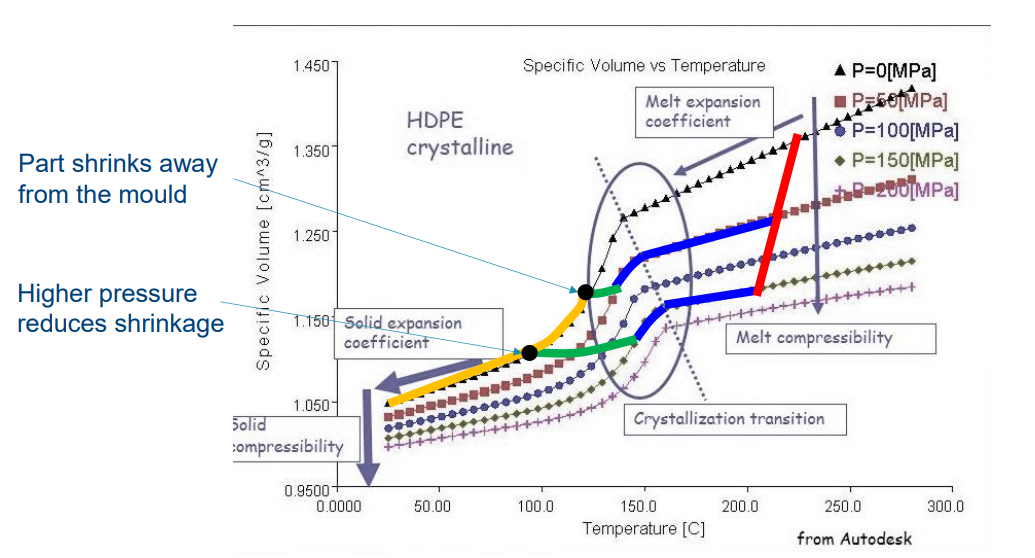
\includegraphics[width=0.8\textwidth]{shrinkage.png}
  \caption{Krimp bij verschillende drukniveaus}
  \label{fig:shrinkage.png}
 \end{figure}
De grafiek hierboven toont verschillende curves voor verschillende drukniveaus, als we een hogere druk uitoefenen op de matrijs zal het specifiek volume kleiner worden en uiteindelijk de krimp ook verminderen. In de grafiek zien we ook een scherpe vertical val in het volume wanneer het materiaal overgaat van 'smelt' naar een vaste kristallijne structuur, dit is de kristallisatie-overgang. Dus als je als ingenieur de krimp wat wilt veranderen kan je een beetje met parameters spelen, dit doe je bevoorbeeld als je toleranties uiteindelijk niet goed zijn.
\subsection{Productieproblemen}
We moeten eigelijk een ideaal werkgebied hebben voor 2 cruciale parameters: de smelttemperatuur en de injectiedruk, anders stoten we op een paar problemen. Het ideale werkgebied wordt weergegeven in de volgende figuur:
\begin{figure}[H]
  \centering
  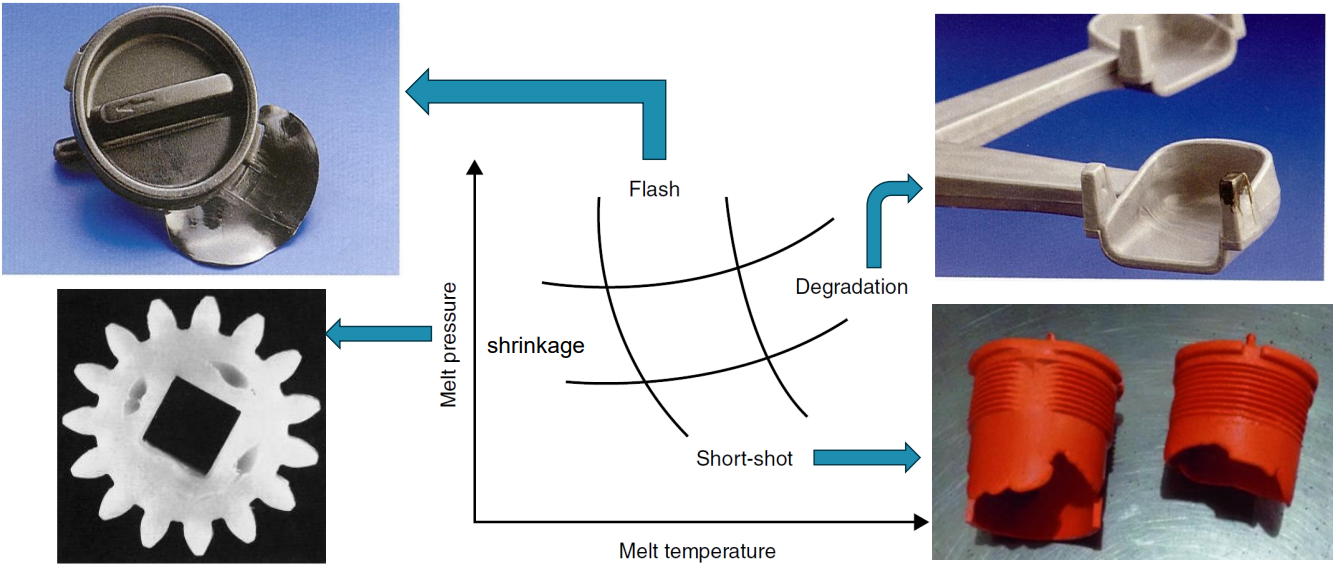
\includegraphics[width=0.8\textwidth]{ideaalwerkgebied.png}
  \caption{Ideaal werkgebied voor smelttemperatuur en injectiedruk}
  \label{fig:ideaalwerkgebied.png}
 \end{figure}
Indien we hierbuiten zitten gaan we op een paar problemen stoten, problemen kunnen zijn:
\begin{itemize}
 \item \textbf{Short shot (ondervulling):} Dit heb je als te weinig materiaal wordt geinjecteerd, of een te lage druk of temperatuur waarbij dit gebeurd, materiaal geraakt niet ver genoeg in de matrijs of stolt te vroeg. Kan je voorkomen met meer injectie volume of hogere injectie druk of temperatuur of een grotere gate of grotere matrijs temperatuur. Lucht uitvoer kanaal grotere maken of meer van maken kan ook helpen.
 \item \textbf{Sink marks (krimpvlekken) en shrinkage voids (krimpgaten):} Dit probleem ontstaat bij dikke secties in het product, de buitenste laag van het onderdeel stolt als eerst maar wanneer het binnenste materiaal daarna afkoelt en krimpt, trekt dit de gestolde buitenste 'huid' naar binnen. Kan je fixen door je CAD-ontwerp aan te passen zodat het een uniforme wanddikte ('wall thickness') heeft, liefst zo dun mogelijk. Ook nog rekening houden met die Fourier-getal! Zie eerder
  \begin{figure}[H]
   \centering
   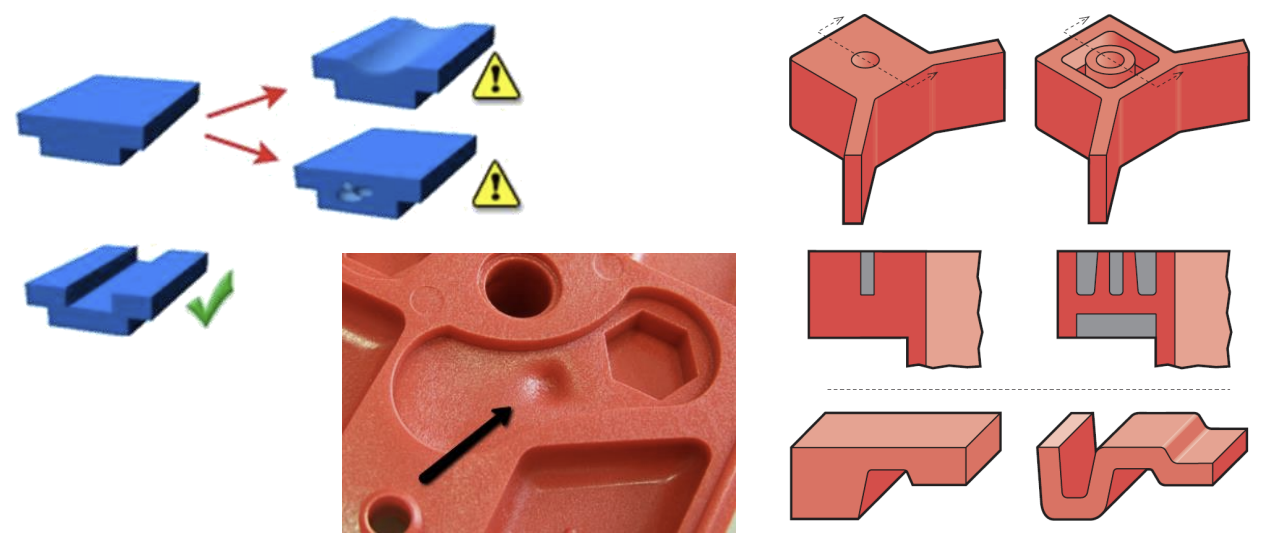
\includegraphics[width=0.8\textwidth]{sinkmarks.png}
   \caption{Foto sink marks}
   \label{fig:sinkmarks.png}
  \end{figure}
 \item \textbf{Burs/Flash (bramen):} Dit is overtollig materiaal dat tussen de sluitende matrijshelften wordt geperst zoals te zien is in de foto:
 \begin{figure}[H]
   \centering
   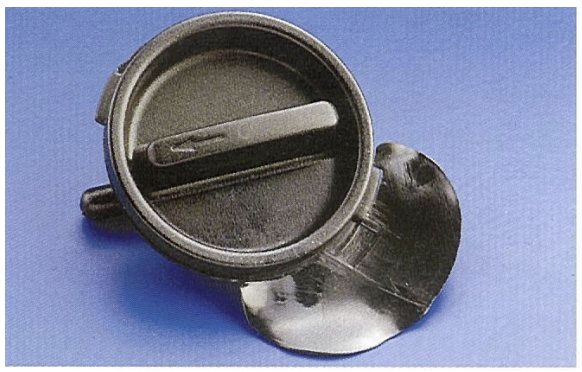
\includegraphics[width=0.4\textwidth]{bursflash.png}
   \caption{Voorbeeld burs/flash}
   \label{fig:bursflash.png}
  \end{figure}
 Dit kan worden veroorzaakt door een te hoge injectiedruk, een te lage viscositeit van het materiaal, een te lage sluitkracht van de machine of simpelweg een ruwe/versleten matrijs. Dus verhoog je sluitkracht, verlaag de injectiesnelheid en materiaaltemperatuur of modificeer de matrijs. In principe kan je bramen achteraf ook wegsnijden maar op grote schaal zorgt dit voor een stijging van productietijd en kosten.
 \item \textbf{Degradatie (diesel effect):} Als de lucht in de caviteit door slechte ontluchting niet kan ontsnappen, wordt die luicht ingesloten en extreem snel adiabatisch gecomprimeerd, dit ontbrandt de lucht wat het polymeer in brand steekt. Dit kan je dus fixen met betere ventilatie in de matrijs of de sluitkracht van de matrijs wat verlagen.
 \begin{figure}[H]
   \centering
   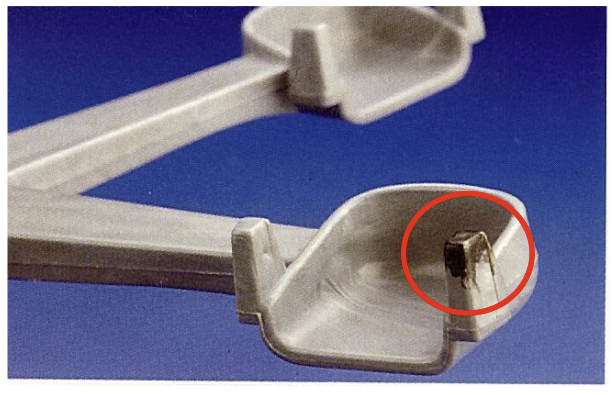
\includegraphics[width=0.4\textwidth]{degradatiediesel.png}
   \caption{Degradatie door het diesel effect}
   \label{fig:degradatiediesel.png}
  \end{figure}
 \item \textbf{Degradatie (verbranding):} Dit is chemische degradatie van het polymeer omdat het te lang op een te hoge temperatuur is gebleven in de schroef of sprue, dit resulteert in visuele defecten (zie foto), dit kan je fixen door de temperatuur of injectiesnelheid te verlagen, de cyclustijd te verkorten en scherpe hoeken te vermijden in het ontwerp, de proff zegt hier ook nog dat als een polymeer degradeert bij verhitting en dat toegevoegde antioxidanten bij elke cyclus verbruikt worden, dit is waarom je polymeren niet eindeloos kunt blijven recycleren.
 \begin{figure}[H]
   \centering
   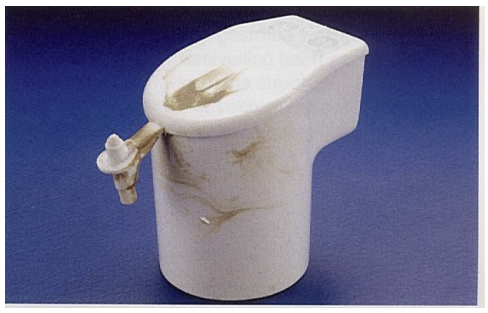
\includegraphics[width=0.4\textwidth]{degradatieburns.png}
   \caption{Degradatie door verbranding}
   \label{fig:degradatieburns.png}
  \end{figure}
 \item \textbf{Ingesloten lucht:} Dit is het resultaat van decompressie: wanneer de zuiger na het injecteren te snel wordt teruggetrokken, wordt er lucht in de matrijsholte gezogen, abrupte geometrische veranderingen of slechte bevochtigingen van de matrijs kunnen hier ook voor zorgen. Dit zorgt dus voor zichtbare luchtbellen in het product. Dit kan gefixt worden met een tragere decompressie en het vermijden van abrupte geometrische veranderingen in het ontwerp.
 \begin{figure}[H]
   \centering
   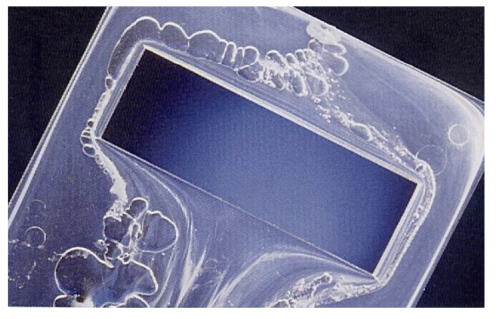
\includegraphics[width=0.4\textwidth]{ingeslotelucht.png}
   \caption{Ingesloten lucht in het product}
   \label{fig:ingeslotelucht.png}
  \end{figure}
 \item \textbf{Weld lines (las lijnen):} Dit is wanneer je 2 'vloeifronten' van gesmolten polymeer elkaar ontmoeten, ze vloeien of mengen dan niet altijd perfect samen ('viskeus materiaal mengt niet zo goed'), en het is als de temperatuur van die fronten te laag is bij het samenkomen dat er een 'laslijn' ontstaat, dit is een zichtbare lijn die ook zorgt voor lokale zwakkere mechanische eigenschappen. Dit kan je fixen door de temperatuur te verhogen en het matrijsontwerp en injectiestrategie te verbeteren. Zorg allesinds dat laslijnen in je ontwerp op niet kritische plekken vallen.
 \begin{figure}[H]
   \centering
   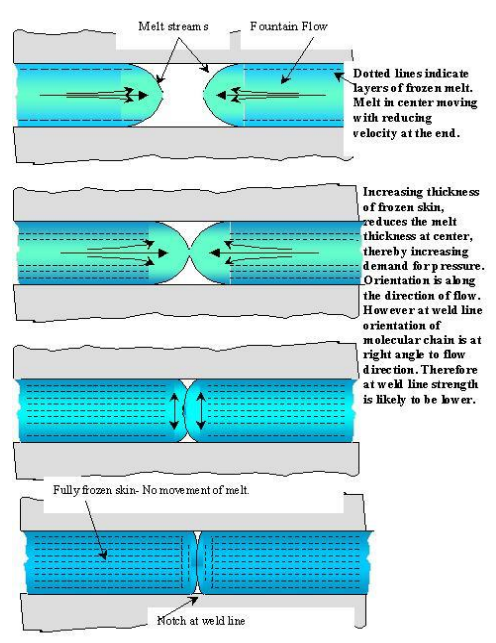
\includegraphics[width=0.5\textwidth]{laslijnen.png}
   \caption{Weld lines in het product}
   \label{fig:laslijnen.png}
  \end{figure}
 \item \textbf{Warping (vervorming):} Dit is het kromtrekken/vervormen van het product, het wordt veroorzakt door de opbouw van 'internal stresses' (thermische spanningen) door temperatuurgradiënten en niet uniforme koeling in de matrijs SAMEN MET 'oriëntatie-effecten' van de polymeerketens TIJDENS het vullen. Van zodra het product is afgekoeld en uit de matrijs wordt gehaald komen die spanningen dus vrij en vervormt het product. Dit is waarom uniform koelen zo belangrijk is.
 \begin{figure}[H]
   \centering
   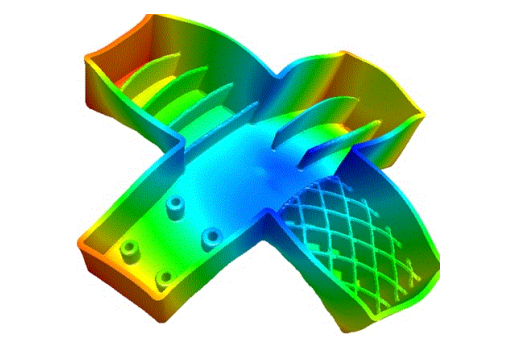
\includegraphics[width=0.4\textwidth]{warping.png}
   \caption{Warping}
   \label{fig:warping.png}
  \end{figure}
\subsubsection{Oriëntatie tijdens injection moulding}
Dit was dus 1 van die oorzaken van warping, het fenomeen gaat als volgt: tijdens het injecteren van het vloeibare polymeer in de matrijs worden de polymeerketens door de stroming (afschuifkrachten) sterk in één richting getrokken, uit de volgende grafiek blijft dat deze oriëntatie in de spuitrichting zeer sterk is aan het oppervlak van het onderdeel (A11). Wat we hier ook opmerken is dat in het midden van het onderdeel (dus binnenin) de oriëntatie meer random is. Het zijn deze oriëntatie-effecten die bijdragen aan die 'internal stresses', een meer willekeurige spreiding in het onderdeel krijgen (wat we dus willen) kunnen we doen door het aanpassen van de injectiestrategie (met de parameters spelen dus). Dit effect heet trouwens ook het 'skin-effect'.
\begin{figure}[H]
  \centering
  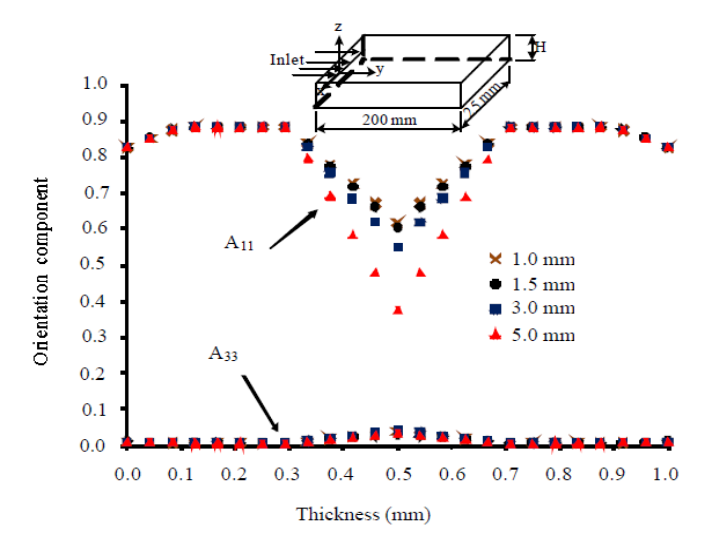
\includegraphics[width=0.5\textwidth]{orientatieeffecten.png}
  \caption{Oriëntatie van polymeerketens tijdens injection moulding}
  \label{fig:orientatieeffecten.png}
 \end{figure}
\subsection{Oplossingen}
\subsubsection{Oplossingen voor koeling}
Dus niet-uniforme koeling zorgt voor warping, dit kunnen we oplossen met 'conformal cooling' (vormvolgende koeling). In plaats van standaard, rechte koelwaterkanalen in de matrijs te boren, ontwerpt men kanalen die perfect de complexe 3D-contouren van het te maken product volgen (zie foto). Hierdoor wordt de warmte overal evensnel afgevoerd in het product, het maken van deze complexe interne koelkanalen wordt gedaan met metaal 3D-printen.
\begin{figure}[H]
  \centering
  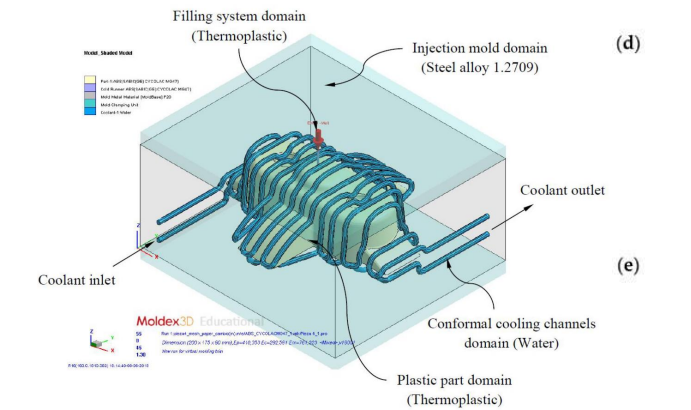
\includegraphics[width=0.5\textwidth]{conformalcooling.png}
  \caption{Vormgevolgde koeling (conformal cooling)}
  \label{fig:conformalcooling.png}
 \end{figure}
\subsubsection{Oplossingen in het productontwerp tegen warping en CAD optimalisatie}
Warping kan voorkomen worden door de geometrie van het product zelf 'slimmer' te maken. Door bevoorbeeld massieve delen te vermijden, symmetrisch ontwerpen (want hierbij heffen opgebouwde krimpspanningen elkaar op tijdens het afkoelen, zie U- of H-vorm) of ribben zetten kan ook soms helpen, een goed CAD-ontwerp heeft altijd uniforme en minimale wanddiktes om cyclustijd en krimpt te beperken, ook zijn er lossingshoeken (draft angles) voorzien om het onderdeel na krimp makkelijk uit de matrijs te krijgen, afronden van hoeken om scherpe hoeken te vermijden moet ook gedaan worden en het CAD-bestand moet eigelijk ook iets groter gemaakt worden voor de matrijs om rekening te houden met krimp.
\begin{figure}[H]
  \centering
  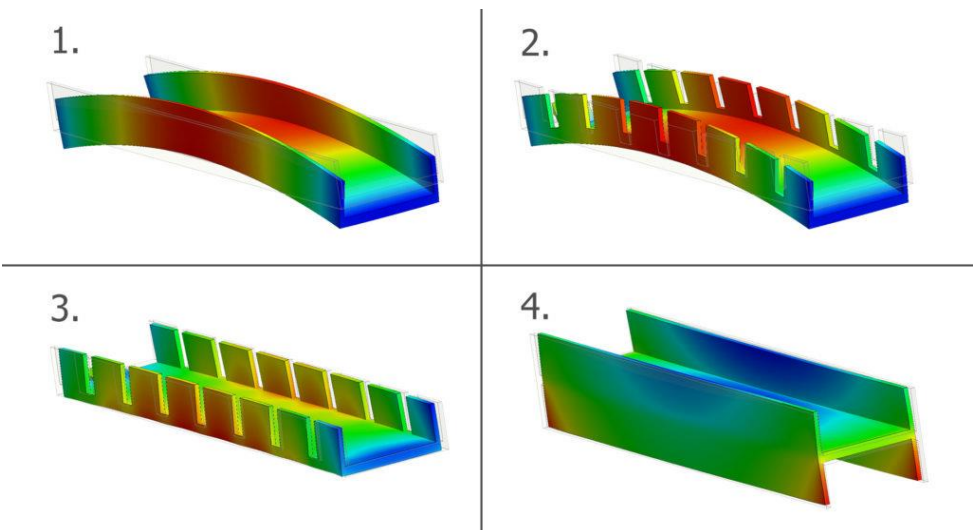
\includegraphics[width=0.6\textwidth]{warpingoptimizing.png}
  \caption{Optimalisatie van het productontwerp tegen warping}
  \label{fig:warpingoptimizing.png}
 \end{figure}
\begin{figure}[H]
  \centering
  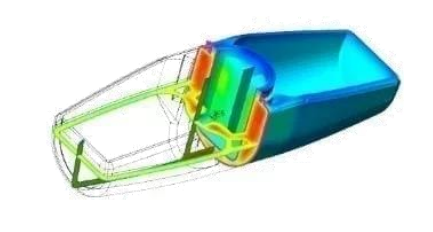
\includegraphics[width=0.5\textwidth]{moldsimulatie.png}
  \caption{CAD Mold simulatie}
  \label{fig:moldsimulatie.png}
 \end{figure}
Het is ook altijd slim om matrijs simulaties te doen in de computer voordat je daadwerkelijk een matrijs produceert, hiermee kan je de effecten van de injectiestrategie simuleren en zien waar laslijnen zullen ontstaan. Warpage door uniformiteit van koeling en verwarming kan ook voorspelt en hierdoor voorkomen worden.
\newpage
\subsection{Additional features (extra functies)}
\subsubsection{Inserts \& Overmoulding (inzetstukken en overgieten)}
Hoe integreren we niet-plastic onderdelen in ons spuitgietproduct?
\newline
Simpel, er wordt een 'insert' gemaakt (van een ander materiaal, meestal een metaal) en dit wordt in de matrijs geplaatst, hierna sluit de matrijs en wordt het plastic er rond gespoten gewoon. Voorbeelden zijn stekkers, handvaken van een metalen tang, \dots
\subsubsection{Multicomponent IM (meerdere componenten spuitgieten)}
Er worden hier nu verschillende materialen (misschien verschillende kleuren) in de matrijs gespoten, bij een tandenborstel wordt dit bevoorbeeld gedaan, het heeft een hard materiaal als stevige ruggengraat en een zacht materiaal als rubberachtig plastic voor een comfortabele grip.
\subsection{Gasinjectiespuitgieten}
Dit wordt gebruikt om holle producten te maken. Eerst wordt de matrijs 'deels' geïnjecteerd met vloeibaar plastic, daarna wordt er onder druk gas (lucht) in de kern van die vloeibare massa gespoten, dit blaast het onderdeel hol en duwt het vloeibaar polymeer stevig tegen de koude wanden van de matrijs aan wardoor het stolt. Voor massieve onderdelen zoals een handvat voor een deur wordt dit bevoorbeeld gedaan, anders heb je sink marks of zou het te lang duren om te koelen, kost dan ook meer materiaal en tijd.
\begin{figure}[H]
  \centering
  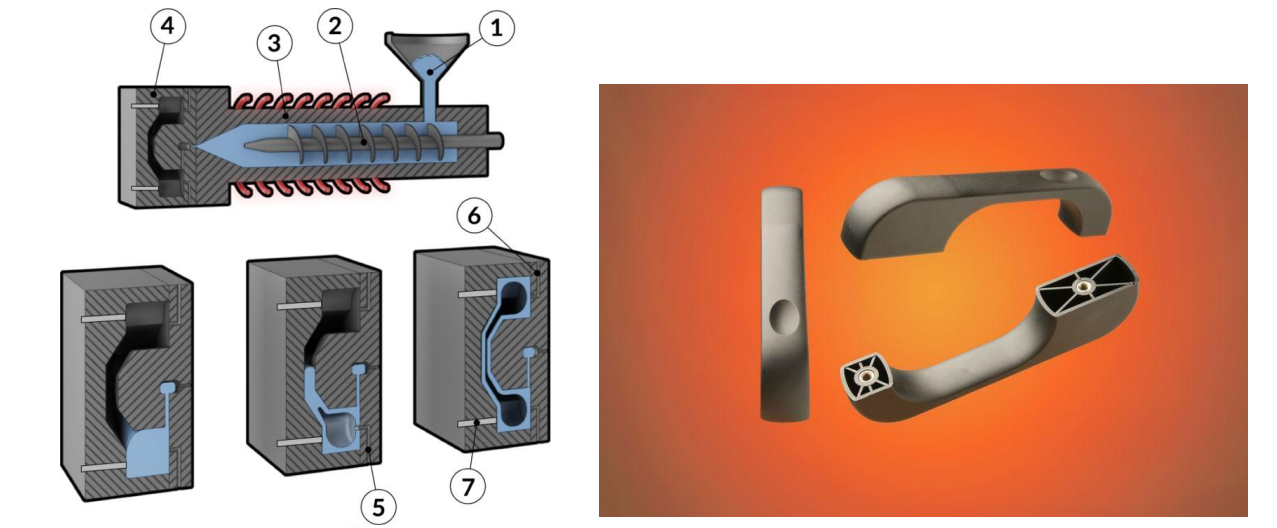
\includegraphics[width=0.6\textwidth]{gasIM.png}
  \caption{Gasinjectiespuitgieten}
  \label{fig:gasIM.png}
 \end{figure}
\begin{warningbox}[Zie slides]
Er staan nog voorbeeldvragen op de slides die we in de les samen hebben bezien, ik heb niet alle antwoorden van deze vragen dus ik zet ze hier niet in. Ook wordt op de slides nog gesproken over 'crystallization', 'effect of cooling rate in amorphous polymers' en 'shrinkage of semi-crystalline polymers' maar dit is niet in de les besproken.
\end{warningbox}
\newpage
\chapter{Processing of thermoplastics (verwerken van thermoplasten)}
\end{itemize}